\section{How many siblings?}
To find the Lot of the Number of Siblings\footnote{Note that \textsl{siblings} is being used here and elsewhere in place of \textsl{brothers}.}, count (in the order of the signs) from \Mercury\, to \Jupiter\, (by night, from \Jupiter\, to \Mercury) and add the difference to the Ascendant. The number of planets aspecting the place of the lot gives you the number of siblings.

Indications from the planets aspecting the place are:
\begin{description}[labelindent=0em , labelwidth=6em, labelsep=0.5em, leftmargin =!]
\item [\Venus,\Mercury] in aspect from a good place, from feminine signs indicates sisters; in masculine signs, brothers

\item[\Saturn,\Mars,\Sun\,\Moon] peregrine, indicate the loss of siblings but if in their own places his siblings ``will not love him and are not his friends or who have no use for him because what the malefics indicate is not complete''

\item[any planet] in aspect from a bad place indicates the siblings ``have no good in them or have sicknesses, or that there is enmity between them, and bad and evil [are their] opinion and thought [of each other]
\end{description}

\subsection{Indications from the 3rd Place}
If the sign on the 3rd place is double-bodied (\Gemini, \Virgo, \Sagittarius, \Pisces) or its lord is in a double-bodied sign then the siblings are not the children of both parents.

Indications from the planets as to birth-order:
\begin{itemize}
\item[\Saturn,\Mars] older brothers
\item[\Jupiter,\Mars] middling brothers
\item[\Mercury] younger brothers
\item[\Moon] older sisters
\item[\Venus] younger sisters
\end{itemize}

\subsection{General Indications from Mars}
If the 1st and 2nd triplicity rulers of \Mars\, are in bad places, it indicates a small number of siblings.

If one triplicity ruler is in  a good place and the other in a bad place then the person has siblings ``but it is inevitable that he will see their death.''

\subsection{An Example Chart}
\vspace{-1em}
\begin{figure}[H]
\centering
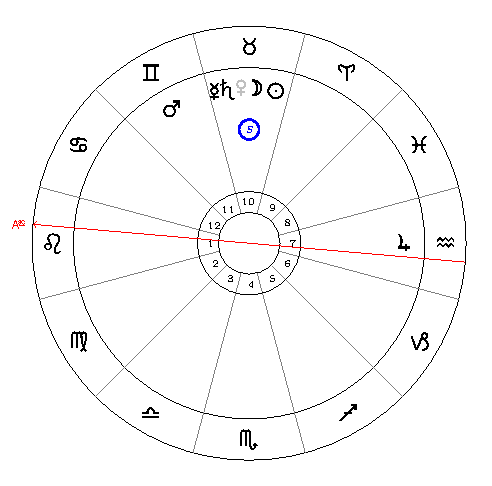
\includegraphics[width=0.7\textwidth]{charts/1_01}
\vspace{-1em}
\caption{Chart 01: Man with 5 Siblings}
\end{figure}

The chart of a man with the \Sun, \Moon, \Saturn, \Mercury\footnote{\Venus\, is missing from the original chart, Dykes places it in the 10th, dating the chart to May 2 or 3, 29 AD JC, $\approx$ 11:30AM Sidon, Lebanon.}, and the Lot of Siblings in the Midheaven in Taurus with \Mars\, in \Gemini, \Jupiter\, in \Aquarius, and the Ascendant in \Leo.

\Saturn\, and \Mercury\, are the indicators of siblings as they are the triplicity rulers of \Mars\, (the general indicator of siblings). ``Because they both happen to be above the earth you count from them to the ascendent, but if they were below the earth you would count from the ascendent to them.''

Predict the person will have five siblings as the two triplicity rulers are in \Taurus\, and counting from there to the ascendent sign of \Leo\, gives: \Taurus\, (1) + \Gemini\, (double-bodied gives 2) + \Cancer\, (1) + \Leo\, (1) = 5.

If both the triplicity rulers had not been in one sign it would be necessary to take the count from whichever was eastern and in a strong place, or, if both were of equal strength, to start the count from the day or night triplicity ruler (depending on the chart sect). 

\subsection{Other Indications from the Lot and Planets}
The Lot of Siblings is in a feminine sign (\Taurus) with \Saturn\, indicating his sister will die, as will both an older and his youngest brothers because the \Sun\, and \Mercury\, are also with the lot and \Saturn\, in \Taurus\, but the fullest effect of these will not be felt because \Jupiter\, aspects the place\footnote{An example of the \Square\, of \Jupiter\, being beneficial rather than harmful when he is angular and in one of his own places (he's the participting triplicity ruler of \Aquarius).}.

Some experts, in predicting the number of siblings, count the planets above the earth in a day chart or below the earth for a night chart. 

If \Jupiter\, or the \Sun\, is with the Lot of Sibling and overcoming the \Moon\, by trine then the person has older brothers.

If \Mercury\, is in the ascendent, say the person has no older brothers or if he did, they are dead.

If the \Moon\, is separating from \Saturn\, in a night chart,  or \Mars\, in a day chart, the persons older brother will die before him and he will have nothing from them other than a remembrance of their eminence.

If the \Moon\, is separating from \Venus, the person has an older sister and he will love the acts of \Venus. He will be better off, in his old age, with respect to his property and medical care,  than he was in his youth.

If the \Moon\, is separating from \Mercury\, the the person is not older than his siblings ``and he is gentle, integral in mind and character for things, and he will be praised concerning this. Look also with this at the varieties of signs as the actualiztion of this will be made clear to you in them.''

If the \Sun\, is in the ascendent there is no good for the person with respect to siblings.

If \Mars\, or \Saturn\, are in the ascendent or midheaven or in the signs following the ascendent or midheaven, it indicates the worst with respect to siblings as the person may have none, or those he has do not survive, or, if they survive, they will be his enemies.

\Mars\, in the 12th, 4th, or 7th means there is no good in the matter of siblings especially if you also find the lord of the Ascendant, or the \Moon\,  is with \Mars\, or \Mars\, is aspecting \Mercury.

\subsection{Indications from the Lot of Fortune}
If the Lot of Fortune and the Lot of Siblings are together the person will benefit from his siblings and inherit their property if they die before him. Say something similar if you find the ruler of Fortune with the Lot of Siblings and (at the same time) the ruler of Siblings  and the ruler of the 3rd place with Fortune.

\subsection{Sibling's Death}
Look at the two lots\footnote{Most probably the Lot of Siblings and the Lot of the Number of Siblings.} and count from them to the body, square or opposition \Saturn, as it indicates when the person is most likely to see the death of his sibling or worse if \Mars\, aspects the place or turns stationary there. \Mars\, being stationary there ``is a calamity'' and moreso if there is no aspect from \Jupiter.

If \Saturn\, and \Mars\,  are in the place of the lot and aspect \Mercury, the death of a younger brother is indicated, if \Venus, the death of a sister.